% define \title (only used by writelatex.com)
%\title{CSEC-793 Project Report_Blank}
%%%%%%%%%%%%%%%%%%%%%%%%%%%%%%%%%%%%%%%%%%%%%%%%%%%%%%%%%%%%%%%%%%%%%%
% LaTeX Template: Project Titlepage
%
% Source: http://www.howtotex.com
% Date: April 2011
% 
% This is a title page template which be used for articles & reports.
% 
% Feel free to distribute this example, but please keep the referral
% to howtotex.com
% 
%%%%%%%%%%%%%%%%%%%%%%%%%%%%%%%%%%%%%%%%%%%%%%%%%%%%%%%%%%%%%%%%%%%%%%
% How to use writeLaTeX: 
%
% You edit the source code here on the left, and the preview on the
% right shows you the result within a few seconds.
%
% Bookmark this page and share the URL with your co-authors. They can
% edit at the same time!
%
% You can upload figures, bibliographies, custom classes and
% styles using the files menu.
%
% If you're new to LaTeX, the wikibook is a great place to start:
% http://en.wikibooks.org/wiki/LaTeX
%
%%%%%%%%%%%%%%%%%%%%%%%%%%%%%%%%%%%%%%%%%%%%%%%%%%%%%%%%%%%%%%%%%%%%%%
%
% --------------------------------------------------------------------
% Preamble
% --------------------------------------------------------------------
\documentclass[ fontsize=11pt,twoside]{scrartcl}	% KOMA

\usepackage[letterpaper,pdftex]{geometry}	% A4paper margins
\setlength{\oddsidemargin}{5mm}			% Remove 'twosided' indentation
\setlength{\evensidemargin}{5mm}

\usepackage[utf8]{ctex}
\usepackage[protrusion=true,expansion=true]{microtype}	
\usepackage{amsmath,amsfonts,amsthm,amssymb}
\usepackage{graphicx}
\usepackage{pseudocode}
\usepackage{multirow}

\usepackage[colorlinks,linkcolor=blue]{hyperref} %超链接

\usepackage[latin1]{inputenc}
\usepackage{tikz}
\usetikzlibrary{shapes,arrows}

\usepackage{listings}
\usepackage{xcolor}
\lstset{
    numbers=left, 
    numberstyle= \tiny, 
    keywordstyle= \color{ blue!70},
    commentstyle= \color{red!50!green!50!blue!50}, 
    frame=shadowbox, % 阴影效果
    rulesepcolor= \color{ red!20!green!20!blue!20} ,
    escapeinside=``, % 英文分号中可写入中文
    xleftmargin=2em,xrightmargin=2em, aboveskip=1em,
    framexleftmargin=2em,
    breaklines=true
} 


% 添加首行缩进,两个字符
\usepackage{indentfirst}
\setlength{\parindent}{2em}

% --------------------------------------------------------------------
% Definitions (do not change this)
% --------------------------------------------------------------------
\newcommand{\HRule}[1]{\rule{\linewidth}{#1}} 	% Horizontal rule

\makeatletter							% Title
\def\printtitle{%						
    {\centering \@title\par}}
\makeatother									

\makeatletter							% Author
\def\printauthor{%					
    {\centering \Large \@author}}				
\makeatother							

% --------------------------------------------------------------------
% Metadata (Change this)
% --------------------------------------------------------------------
\title{	\Large \textsc{编译原理课程实验 \\ 
															实验报告} 	% Subtitle
		 	\\[2.0cm]								% 2cm spacing
			\HRule{2pt} \\						% Upper rule
			\LARGE \textbf{\uppercase{SEULex 实验报告}}	% Title
			\HRule{2pt} \\ [0.5cm]		% Lower rule + 0.5cm spacing
			\Large 2021年1月20日			% Todays date
		}

 \author{
		71118313 张晓铮\\	
		东南大学软件学院\\
}


\begin{document}
% ------------------------------------------------------------------------------
% Maketitle
% ------------------------------------------------------------------------------
\thispagestyle{empty}		% Remove page numbering on this page

\printtitle					% Print the title data as defined above
  	\vfill
\printauthor				% Print the author data as defined above
\newpage
% Make contents
\pagenumbering{roman}
\tableofcontents
\newpage
% ------------------------------------------------------------------------------
% Begin document
% ------------------------------------------------------------------------------
\pagenumbering{arabic}
\setcounter{page}{1}		% Set page numbering to begin on this page

\co

%%%%%%%%%%%%%%%
%														%
% 			Main Contents            %
%														%
%%%%%%%%%%%%%%%
\section{实验目标}
本次实验的目标为开发一个利用软编码的方式,可以解析用户指定格式文件的Lexer和Parser,其中对于词法和语法的DFA和LR Table由用户自己生成,本程序只根据用户输入的DFA和LR Table进行相应的解析
\section{实验环境}
\begin{itemize}
    \item 本次实验采用的实验环境:
    \begin{itemize}
        \item[1]操作系统:Windows 10
        \item[2]语言:Java 14
    \end{itemize}
\end{itemize}
\section{实验内容}
\begin{itemize}
    \item 主要内容
    \begin{itemize}
        \item[1]读取用户输入的DFA和LR Table,并利用合适的数据结构存储起来
        \item[2]编写读入源文件以及根据DFA和LR Table解析的程序
    \end{itemize}
\end{itemize}

\section{实验实现方法}
在本次实验中,由于DFA和LR Table最终都可以用一张表来表示,所以采用csv文件来存储用户输入的LR Table和DFA,以实现软编码的目的。然后根据读入的表进行解析,首先用Lexer读入用户输入的源文件,一次读入一个字符,并在DFA上进行状态之间的转换,并适当的进行报错处理。Lexer提供了next函数,每次返回一个Token类,用来表示识别到的词,然后交由Parser处理,Parser根据传入的Token和LR Table进行状态的移动,最终形成一棵Parser Tree
\subsection{SoftCodeLexer关键内容描述}
\subsubsection{State}
该类主要内容为String name,boolean isAcceptState以及HashMap<String, String> mapping2statename;它们分别记录了当前状态的名称,是否为结束节点,以及该状态能经过什么符号到达下一个状态的名称;


并且提供了方法getNextStateName,它能根据传入的字符寻找能到达的状态的名称并返回,如果没有则返回null
\subsubsection{DFA}
该类主要保存用户输入的DFA,其中关键的数据成员为:HashMap<String, State> name2state,该map用于记录所有的State并将它们的名称和状态做映射;State start用于记录开始状态;State currentState用于DFA在状态之间转换时记录当前所在的状态;


该类提供了next函数,它接受一个字符,并判断能否从当前状态经过这个字符到达另一个状态,如果不可以则返回false,可以的话返回true;同时提供了函数isAcceptingState,用来判断当前状态是否是accept的,还提供了returnToStart函数,用于将DFA的当前状态重置到开始状态。


对DFA做这样的封装,可以让外部使用者只调用next,判断是否是accepting的即可,对于DFA内部的状态是如何转换的可以不关心。

\subsubsection{Token}
该类用于表示词法分析器生成的Token,主要含有Long id, String type, String lexValue,分别表示该Token的id,类型和对应的解析出来的真实值。其中type为用户在配置文件中自己定义的名称。
\subsubsection{Lexer}
该类为实现词法分析的类,它使用封装好的DFA,并维护了一个char[] buf,buffer的大小可由用户配置,其工作流程为每次读入buffer大小的字符,对字符进行遍历,遍历一个字符将其交给DFA,如果DFA返回false,说明不能继续走,然后判断DFA当前状态能否接受,如果能则输出,不能则报错。

\subsection{SoftCodeParser关键内容描述}
\subsubsection{Expression}
该类主要用于存储用户输入的语法产生式,由于我们要求的产生式为上下文无关文法,所以该类用一个String leftPart存储产生式的左部,而右部用ArrayList<String> rightPart来按照顺序存储
\subsubsection{Grammar}
该类用于存储所有的产生式,它使用一个HashMap<String, Expression> allExpression将用户定义的产生式名称和产生式相关联并存储,并提供了按照名称返回产生式的方法。
\subsubsection{LRTableRow}
该类用于存储LR Table中的一行,类似于DFA中的状态,它主要含有两个数据成员:HashMap<String, Pair<String, Integer>> actions,用来存储action表,它将表示该状态能从哪种Token转移到下一个状态或用什么来规约,Pair<String, Integer>种用Integer表示是移进还是规约还是到达了accept状态,如果是移进,则Pair中第一个String表示要移进的状态名,如果是规约或者accept则表示产生式的名称;HashMap<String, String> goto表示goto表,表示能从哪个非终结状态到达哪个状态;String name代表当前行的状态名称。
\subsubsection{LRTable}
该类用来存储完整的LRTable,利用HashMap<String, LRTableRow> rows存储所有行,并将每行的状态的名称和该行做映射,并提供了canReach和canGoto函数用来判断通过给定的终结符或非终结符的下一步状态,如规约,移进或accept。
\subsubsection{ParserTreeNode}
该类是生成的语法分析树的节点,保存了int id,boolean isLeaf表示是否为叶节点,String symbol表示对应Token的type,String value表示如果是叶节点则它的lexValue是多少,以及List<ParserTreeNode>表示它的儿子节点
\subsubsection{ParserTree}
该类保存了ParserTree的根节点
\subsubsection{Parser}
该类为语法分析器的核心,它使用了Lexer和LRTable,parser函数为解析函数,它每次读入Lexer的一个字符,同时维护符号栈和状态栈,根据Token的type查LRTable决定下一步动作:如果是移入则创建新的ParserTreeNode,将Token中的lexValue放入,并令其为叶节点,压入符号栈;如果规约则相应的将符号栈中的符号弹出与Grammar中的Expression比较能否成功规约,并创建新的ParserTreeNode,其不是叶节点,并且儿子节点为符号栈中弹出的可规约的ParserTreeNode,规约完成后将这个节点压入符号栈,并根据goto表查找正确的状态名称压入状态栈。


这样在规约结束时即可获得一棵语法分析树。
\section{实验结果}
可执行代码见源码,使用方法见源码中的README,源码可从github上查看下载,地址https://github.com/zhang-x-z/CompilerPrincipal-Lab


测试选取了解析JSON文件中的Token,包括string,\{,\},number,[,],:,逗号,true,null,false以及空格(包括制表符换行),输入的xml文件如下
\begin{lstlisting}
<?xml version="1.0" encoding="UTF-8"?>
<Lex>
    <userDefinitions></userDefinitions>
    <reDefinitions>
        <digit>
            [0-9]
        </digit>
    </reDefinitions>
    <rules>
        <rule>
            <re>
                "(\\.|[^\\"\n])*"
            </re>
            <action>
                cout &lt;&lt; "STRING" &lt;&lt; endl;
            </action>
        </rule>
        <rule>
            <re>
                \{
            </re>
            <action>
                cout &lt;&lt; "LEFT BRACE" &lt;&lt; endl;
            </action>
        </rule>
        <rule>
            <re>
                }
            </re>
            <action>
                cout &lt;&lt; "RIGHT BRACE" &lt;&lt; endl;
            </action>
        </rule>
        <rule>
            <re>
                ,
            </re>
            <action>
                cout &lt;&lt; "COMMA" &lt;&lt; endl;
            </action>
        </rule>
        <rule>
            <re>
                :
            </re>
            <action>
                cout &lt;&lt; "COLON" &lt;&lt; endl;
            </action>
        </rule>
        <rule>
            <re>
                \[
            </re>
            <action>
                cout &lt;&lt; "LEFT BRACKET" &lt;&lt; endl;
            </action>
        </rule>
        <rule>
            <re>
                ]
            </re>
            <action>
                cout &lt;&lt; "RIGHT BRACKET" &lt;&lt; endl;
            </action>
        </rule>
        <rule>
            <re>
                [\r\t \n]
            </re>
            <action>
                cout &lt;&lt; "WIGHTSPACE" &lt;&lt; endl;
            </action>
        </rule>
        <rule>
            <re>
                [1-9]{digit}*|0
            </re>
            <action>
                cout &lt;&lt; "INT" &lt;&lt; endl;
            </action>
        </rule>
        <rule>
            <re>
                ([1-9]{digit}*\.{digit}*)|(0\.{digit}*)
            </re>
            <action>
                cout &lt;&lt; "FLOAT" &lt;&lt; endl;
            </action>
        </rule>
        <rule>
            <re>
                true
            </re>
            <action>
                cout &lt;&lt; "TRUE" &lt;&lt; endl;
            </action>
        </rule>
        <rule>
            <re>
                false
            </re>
            <action>
                cout &lt;&lt; "FALSE" &lt;&lt; endl;
            </action>
        </rule>
        <rule>
            <re>
                null
            </re>
            <action>
                cout &lt;&lt; "NULL" &lt;&lt; endl;
            </action>
        </rule>
    </rules>
    <userCode></userCode>
</Lex>
\end{lstlisting}
配置文件如下
\begin{lstlisting}
buffer_size=60
source_file_location=./test.xml
encoding=utf8
charset=ascii
\end{lstlisting}
测试用JSON文件:
\lstset{language=json}
\begin{lstlisting}
{
    "name": "ZXZ",
    "age": 21,
    "GPA": 3.92,
    "is_male": true,
    "is_famale": false,
    "courses": [
        "Database", "CompilePrincipal", null
    ]
}
\end{lstlisting}
最后输出结果如图:\\
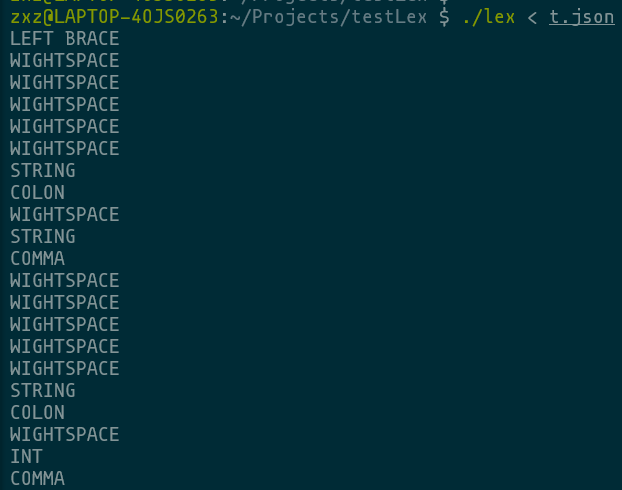
\includegraphics[scale=0.8]{1.png}\\
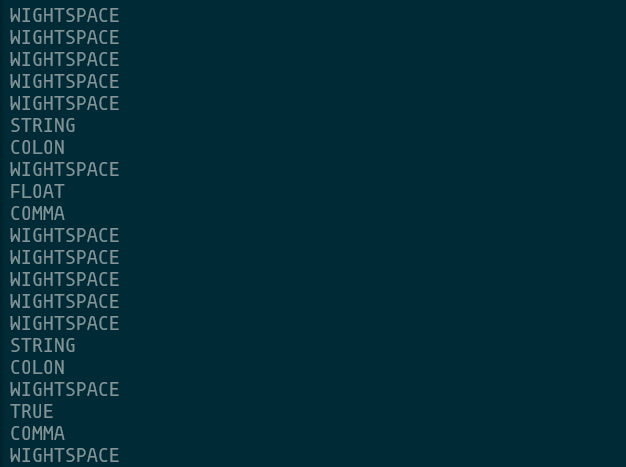
\includegraphics[scale=0.8]{2.png}\\
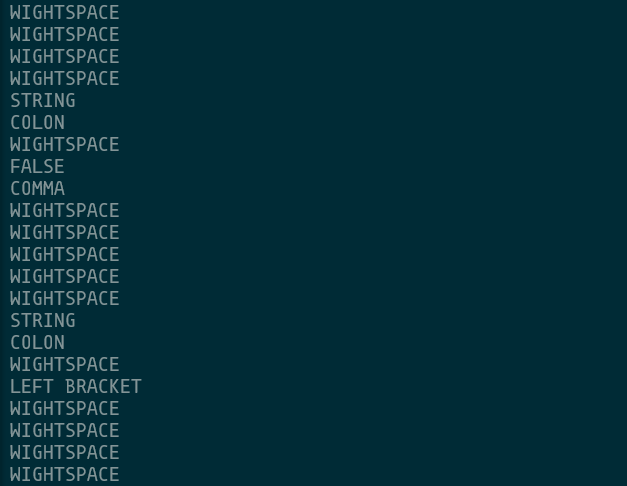
\includegraphics[scale=0.8]{3.png}\\
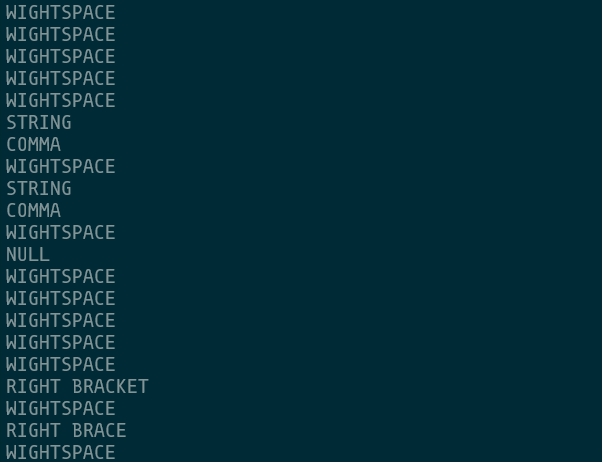
\includegraphics[scale=0.8]{4.png}
\section{实验小结}
通过本次实验,对编译原理中的词法分析部分有了较深的理解。在实验过程中,一开始遇到的阻力很大,比如最开始的.l文件的读取处理,由于不想在这个部分花费太多时间,想把精力集中在后面的算法部分,就利用xml文件来组织用户输入的正规表达式,并利用第三方库来解析。同时对于正规表达式规范化部分也遇到了很多问题,甚至去github上查看了flex的源代码,最后利用自己规定的正规表达式规则,并且用字符串的搜索匹配方法,对正规表达式不断扫描,每次扫描进行一种处理,最终将正规表达式转换为规范化的正规表达式。


对于中缀转后缀,后缀转NFA和NFA转DFA以及DFA最小化,有确定的算法,写起来比较轻松。

此外还遇到的一个问题就是对于字符的处理,因为我希望这个程序能处理多种字符,而不只是处理ASCII中的字符,所以提供了一个charset的接口,可以让用户自己配置自己词法分析器中的字符集,比如可以配置UNICODE字符集等,但由于时间精力的原因,目前只提供了ASCII的字符集实现,但由于使用了接口,使得程序易于扩展,只要添加相应的实现类以及配置选项即可。
% ------------------------------------------------------------------------------
% End document
% ------------------------------------------------------------------------------
\end{document}